

\section{The mean temperature of each year}
The general structure that I used to preform this task was the suggested with a class called tempTrender. Therefore a header file where the class is declared was used. The file $\textbf{tempTrender.cpp}$ contains the implementations of the constructor and method used for my task.  Instead of using the $\textbf{project.cpp}$ file the function within the file was moved to a common file for all group members. This function creates an instance of the class, and runs the method  $\textbf{tempPerYear}$ for that instance. 


The wanted result is plots of histograms with the average temperature of each year. The first thing that needs to be done is to read in the data file. This was done in the implementation of the constructor in  $\textbf{tempTrender.cpp}$. After that the wanted data needs to be extracted from the file.  Looping over all strings, and with various if statements, the wanted data could be selected. Since this project wants the average yearly temperature, only the year that are completed were used. Also in some files there are only data points from 06.00 and 18.00 at later years, while at the start of the measurement there were three at 06.00, 12.00 and 18.00. To solve this only the data points from 06.00 and 18.00 were used. The temperature values were assigned to an array, were each data point corresponds to a year. A counter for the number of temperature measurements per year was also used. With these two a yearly average temperature could be calculated. Also the mean of the average yearly temperature from all the years could be calculated. 

In the method  $\textbf{tempPerYear}$ a histogram of the average yearly temperature was made. After that a histogram of the mean of the average yearly temperature. A third histogram with either the mean of the average yearly temperature or average yearly temperature, depending on if it is larger or smaller then the mean of the average yearly temperature, was also made. These are to create the deviation from average effect that was requested. Together with these two lines can be seen. The black line is the moving average, which takes the closest 5 points including the year itself. The green line is a fitted $\arctan$ function. An $\arctan$ function was chosen because it seems to fit the data well. Since an increase around late 1980s can be seen, the $\arctan=0$ was set at 1987. Because of the chosen function to fit the data to, a unrealistic value for the mean temperature of year 2050 was calculated to 8.3$^{\circ}$C. Although one could argue that more could not be concluded from the current data. 

As the code was made to be able to handle any of the datasets but Uppsala. Lund is shown in the figure below. 

	

\begin{figure}
    \centering
		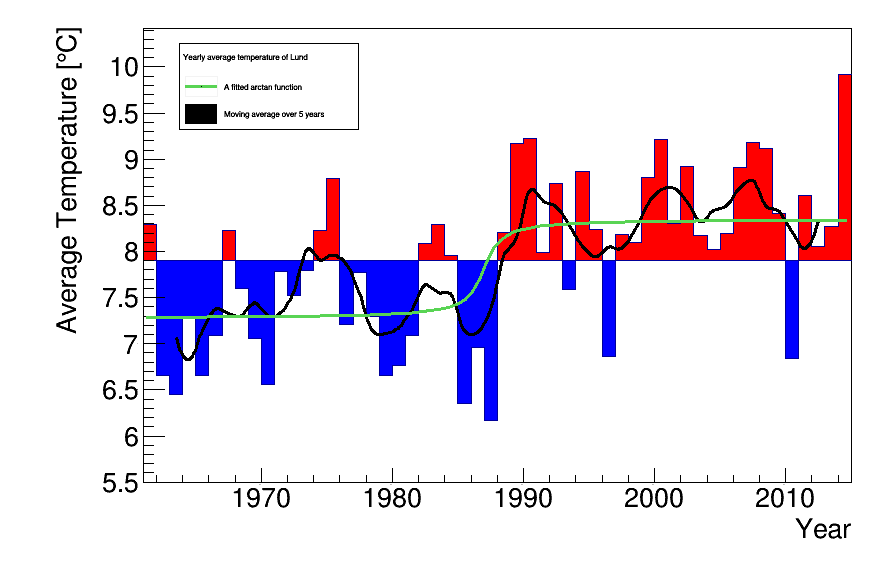
\includegraphics[width=14cm]{yearAvg_Lund.png}
		\caption{Yearly average temperature of Lund}
		\label{Lund}
\end{figure}

\end{document}
